\documentclass{beamer}
\usepackage{tikz}
\usepackage[utf8]{inputenc}
\usetikzlibrary{trees}

% Daniel's proposal for "uncovering" parts of a tikz-tree %
\tikzset{
  invisible/.style={opacity=0},
  visible on/.style={alt=#1{}{invisible}},
  alt/.code args={<#1>#2#3}{%
    \alt<#1>{\pgfkeysalso{#2}}{\pgfkeysalso{#3}} % \pgfkeysalso doesn't change the path
  },
}    

\begin{document}
\begin{frame}
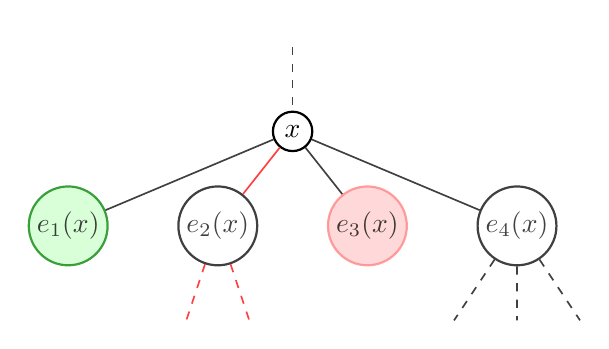
\begin{tikzpicture}[
ball/.style={circle, thick, solid,inner sep=0.5mm, minimum size=5mm},
nor/.style={ball,draw=black,fill=none},
acc/.style={ball,draw=green!50!black,fill=green!20},
rej/.style={ball,draw=red!50,fill=red!20},
level 1/.style={every child/.style={edge from parent/.style={dashed,draw,nearly opaque, visible on=<2->}}},
level 2/.style={sibling distance=19mm,every child/.style={edge from parent/.style={solid,draw,visible on=<2->}}},
level 3/.style={sibling distance=8mm,every child/.style={edge from parent/.style={dashed,draw,nearly opaque, visible on=<5->}} },
semithick]

\node[draw=none] (root) {}
  child[level distance=12mm,visible on=<1->] { node[nor] {$x$}
    child[visible on=<2->] {node[acc] {$e_1(x)$} }
    child[visible on=<3->] {node[nor] {$e_2(x)$} edge from parent[red, visible on=<4->]
      child[visible on=<6->] child[visible on=<6->] }
    child[visible on=<2->] {node[rej] {$e_3(x)$} }
    child[visible on=<3->] {node[nor] {$e_4(x)$}
      child[visible on=<6->] {} child[visible on=<6->] child[visible on=<6->] }
  };
\end{tikzpicture}
\end{frame}
\end{document}